%%
%% This is file `sample-sigplan.tex',
%% generated with the docstrip utility.
%%
%% The original source files were:
%%
%% samples.dtx  (with options: `sigplan')
%% 
%% IMPORTANT NOTICE:
%% 
%% For the copyright see the source file.
%% 
%% Any modified versions of this file must be renamed
%% with new filenames distinct from sample-sigplan.tex.
%% 
%% For distribution of the original source see the terms
%% for copying and modification in the file samples.dtx.
%% 
%% This generated file may be distributed as long as the
%% original source files, as listed above, are part of the
%% same distribution. (The sources need not necessarily be
%% in the same archive or directory.)
%%
%% Commands for TeXCount
%TC:macro \cite [option:text,text]
%TC:macro \citep [option:text,text]
%TC:macro \citet [option:text,text]
%TC:envir table 0 1
%TC:envir table* 0 1
%TC:envir tabular [ignore] word
%TC:envir displaymath 0 word
%TC:envir math 0 word
%TC:envir comment 0 0
%%
%%
%% The first command in your LaTeX source must be the \documentclass command.

\documentclass[sigplan]{acmart}
%% NOTE that a single column version is required for 
%% submission and peer review. This can be done by changing
%% the \doucmentclass[...]{acmart} in this template to 
%% \documentclass[manuscript,screen,review]{acmart}
%% 
%% To ensure 100% compatibility, please check the white list of
%% approved LaTeX packages to be used with the Master Article Template at
%% https://www.acm.org/publications/taps/whitelist-of-latex-packages 
%% before creating your document. The white list page provides 
%% information on how to submit additional LaTeX packages for 
%% review and adoption.
%% Fonts used in the template cannot be substituted; margin 
%% adjustments are not allowed.
%%
%% \BibTeX command to typeset BibTeX logo in the docs
\AtBeginDocument{%
  \providecommand\BibTeX{{%
    \normalfont B\kern-0.5em{\scshape i\kern-0.25em b}\kern-0.8em\TeX}}}

%% Rights management information.  This information is sent to you
%% when you complete the rights form.  These commands have SAMPLE
%% values in them; it is your responsibility as an author to replace
%% the commands and values with those provided to you when you
%% complete the rights form.
%\setcopyright{acmcopyright}
%\copyrightyear{2018}
%\acmYear{2018}
%\acmDOI{XXXXXXX.XXXXXXX}




%%
%% Submission ID.
%% Use this when submitting an article to a sponsored event. You'll
%% receive a unique submission ID from the organizers
%% of the event, and this ID should be used as the parameter to this command.
%%\acmSubmissionID{123-A56-BU3}

%%
%% For managing citations, it is recommended to use bibliography
%% files in BibTeX format.
%%
%% You can then either use BibTeX with the ACM-Reference-Format style,
%% or BibLaTeX with the acmnumeric or acmauthoryear sytles, that include
%% support for advanced citation of software artefact from the
%% biblatex-software package, also separately available on CTAN.
%%
%% Look at the sample-*-biblatex.tex files for templates showcasing
%% the biblatex styles.
%%

%%
%% The majority of ACM publications use numbered citations and
%% references.  The command \citestyle{authoryear} switches to the
%% "author year" style.
%%
%% If you are preparing content for an event
%% sponsored by ACM SIGGRAPH, you must use the "author year" style of
%% citations and references.
%% Uncommenting
%% the next command will enable that style.
%%\citestyle{acmauthoryear}

%%
%% end of the preamble, start of the body of the document source.
\setcopyright{none}%remueve el copyright
\settopmatter{printacmref=false} % remueve la citación
\renewcommand\footnotetextcopyrightpermission[1]{} %remueve el bottom footnote

\renewcommand{\contentsname}{Índice}
\renewcommand{\keywordsname}{Palabras clave}
\captionsetup[table]{name=Tabla} % Set table name to "Table"
\captionsetup[figure]{name=Figura} % Set figure name to "Figure"

\begin{document}

%%
%% The "title" command has an optional parameter,
%% allowing the author to define a "short title" to be used in page headers.
\title{Data Profiling}
\subtitle{Calidad de Datos y Big Data en Ingeniería de Software}
%%
%% The "author" command and its associated commands are used to define
%% the authors and their affiliations.
%% Of note is the shared affiliation of the first two authors, and the
%% "authornote" and "authornotemark" commands
%% used to denote shared contribution to the research.
\author{Alejandro Adorjan}
\email{adorjan@ort.edu.uy}
\orcid{0000-0002-5257-284X}



%%
%% By default, the full list of authors will be used in the page
%% headers. Often, this list is too long, and will overlap
%% other information printed in the page headers. This command allows
%% the author to define a more concise list
%% of authors' names for this purpose.
%\renewcommand{\shortauthors}{Trovato and Tobin, et al.}

%%
%% The abstract is a short summary of the work to be presented in the
%% article.
\begin{abstract}
El objetivo de este trabajo es realizar un informe respecto de las siguientes tareas: 
\begin{enumerate}
    \item Data profiling de tres archivos de datos publicados.
    \item Especificación de un modelo de calidad de datos que cubra algounos de esos datos. Se deberá priorizar que aspectos y que datos se van a evaluar. Justificación. 
    \item Especificación de la base de datos donde se almacenarán las medidas de calidad obtenidas en la medición. 
    \item Ejecución de la medición de calidad. 
    \item Evaluación final de calidad. Análisis de resultados de medición. Niveles de calidad esperados.
\end{enumerate}
\end{abstract}
\settopmatter{printacmref=false}
%%
%% The code below is generated by the tool at http://dl.acm.org/ccs.cfm.
%% Please copy and paste the code instead of the example below.
%%
%\begin{CCSXML}
%<ccs2012>
% <concept>
%  <concept_id>10010520.10010553.10010562</concept_id>
%  <concept_desc>Computer systems organization~Embedded systems</concept_desc>
%  <concept_significance>500</concept_significance>
% </concept>
% <concept>
%  <concept_id>10010520.10010575.10010755</concept_id>
%  <concept_desc>Computer systems organization~Redundancy</concept_desc>
%  <concept_significance>300</concept_significance>
% </concept>
% <concept>
%  <concept_id>10010520.10010553.10010554</concept_id>
%  <concept_desc>Computer systems organization~Robotics</concept_desc>
%  <concept_significance>100</concept_significance>
% </concept>
% <concept>
%  <concept_id>10003033.10003083.10003095</concept_id>
%  <concept_desc>Networks~Network reliability</concept_desc>
%  <concept_significance>100</concept_significance>
% </concept>
%</ccs2012>
%\end{CCSXML}

%\ccsdesc[500]{Computer systems organization~Embedded systems}
%\ccsdesc[300]{Computer systems organization~Redundancy}
%\ccsdesc{Computer systems organization~Robotics}
%\ccsdesc[100]{Networks~Network reliability}

%%
%% Keywords. The author(s) should pick words that accurately describe
%% the work being presented. Separate the keywords with commas.
\keywords{data profiling, data quality, big data}

%% A "teaser" image appears between the author and affiliation
%% information and the body of the document, and typically spans the
%% page.
%\begin{teaserfigure}
 % 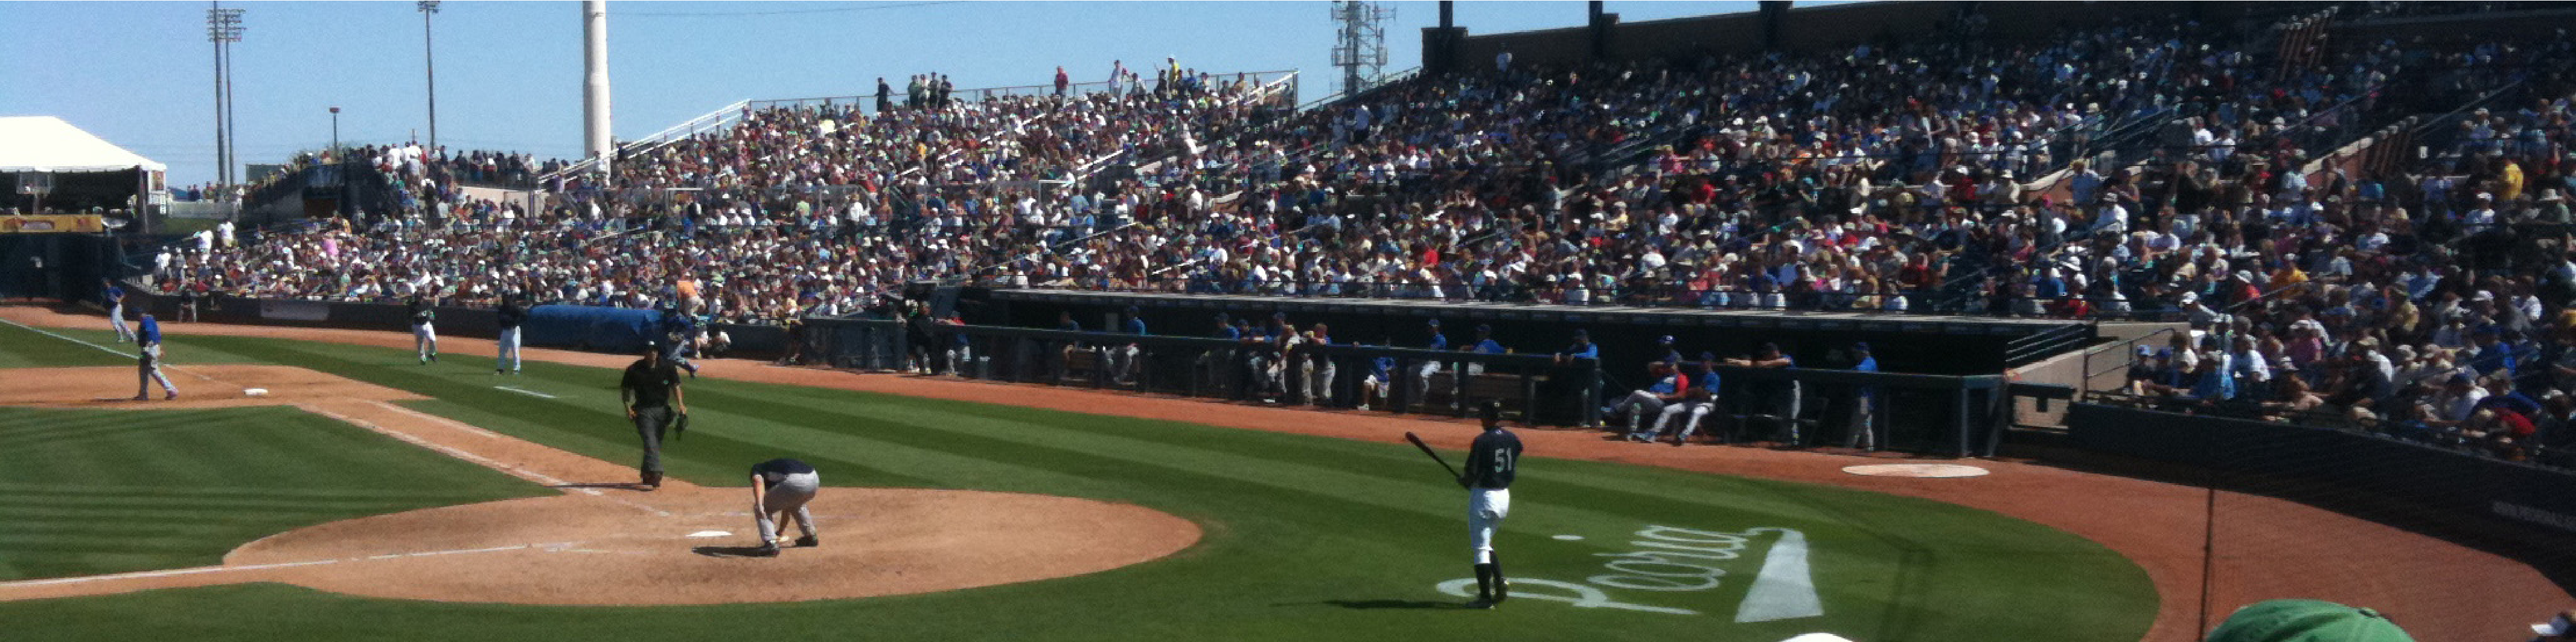
\includegraphics[width=\textwidth]{sampleteaser}
  %\caption{Seattle Mariners at Spring Training, 2010.}
  %\Description{Enjoying the baseball game from the third-base
  %seats. Ichiro Suzuki preparing to bat.}
  %\label{fig:teaser}
%\end{teaserfigure}

%\received{20 February 2007}
%\received[revised]{12 March 2009}
%\received[accepted]{5 June 2009}

%%
%% This command processes the author and affiliation and title
%% information and builds the first part of the formatted document.
\maketitle


\tableofcontents


%---------------------------------------------
\section{Introducción}
\label{sec:intro}
%---------------------------------------------
\subsection{Data Profiling}

"El proceso de descubrimiento de metadatos se conoce como ``data profiling''. Las actividades de ``data profiling'' van desde enfoques ``ad-hoc'', como subconjuntos aleatorios de datos, formulación de consultas de agregación, hasta la inferencia sistemática de información estructural y estadísticas de un conjunto de datos utilizando perfiles dedicados y herramientas
\cite{abedjan2017data}. La elaboración de ``data profiling'' es el conjunto de actividades y procesos para determinar los metadatos sobre un conjunto de datos determinado. Entre los resultados mas frecuentes se encuentran el establecer estadísticas por columna, como la cantidad de valores nulos y valores distintos en una columna, su tipo de datos o los patrones más frecuentes de sus valores de datos. La creación de ``data profiling'' juega un papel importante en distintos casos de uso, como ser la exploración,  integración, y el análisis de datos \cite{abedjan2018introduction}. El objetivo de la elaboración de``data profiling''  mide la consistencia y precisión de los datos, detectando duplicaciones de los mismos para obtener el valor correcto de los datos que podrían usarse en la toma de decisiones \cite{elbaghazaoui2021data}.

\subsection{Modelo de Calidad}

ISO/IEC 25012 define modelo de calidad de datos como ``un modelo general de calidad de datos para datos retenidos en un formato estructurado dentro de un sistema informático. Se centra en la calidad de los datos como parte de un sistema informático y define las características de calidad de los datos de destino utilizados por los seres humanos y los sistemas''. \footnote{\url{https://iso25000.com/index.php/en/iso-25000-standards/iso-25012}}.



\begin{table*}
  \caption{ISO/IEC 25012}
  \label{tab:modelo}
  \begin{tabular}{lp{8cm}}
    \toprule
    Característica &Definición\\
    \midrule
    \textbf{Exactitud | Accuracy} & Grado en el que los datos tienen atributos que permiten ser leídos e interpretados por los usuarios y son expresados utilizando lenguajes, símbolos y unidades apropiados en un contexto de uso específico. Cierta información sobre la comprensibilidad puede ser expresada mediante metadatos.`` \textbf{Exactitud Sintáctica}: cercanía de los valores de los datos a un conjunto de valores definidos en un dominio considerado sintácticamente correcto. \textbf{Exactitud Semántica}: cercanía de los valores de los datos a un conjunto de valores definidos en un dominio considerado semánticamente correcto.
\\
    \textbf{Completitud | Completeness} & Grado en el que los datos asociados con una entidad tienen valores para todos los atributos esperados e instancias de entidades relacionadas en un contexto de uso específico. \\
\textbf{Consistencia | Consistency} & Grado en el que los datos están libres de contradicción y son coherentes con otros datos en un contexto de uso específico. Puede ser analizada en datos que se refieran tanto a una como a varias entidades comparables. \\
\textbf{Comprensibilidad | Understandability } & Grado en el que los datos tienen atributos que permiten ser leídos e interpretados por los usuarios y son expresados utilizando lenguajes, símbolos y unidades apropiados en un contexto de uso específico. Cierta información sobre la comprensibilidad puede ser expresada mediante metadatos. \\

  \bottomrule
\end{tabular}
\end{table*}


%\verb|acmconf|}: The default proceedings template style.
% verb|sigchi|}: Used for SIGCHI conference articles.
%\verb|sigchi-a|}: Used for SIGCHI ``Extended Abstract'' articles.
%sigplan|}: Used for SIGPLAN conference articles.
\section{Reporte}

En esta sección se describen los principales puntos establecidos por el objetivo del trabajo. 
\label{sec:report}
\subsection{Data Profiling de los 3  archivos publicados}

\subsubsection{Fuente de datos}
En el siguiente repositorio
\href{https://github.com/aadorian/cibse_taller.git}{\url{https://github.com/aadorian/cibse_taller.git}}
están disponibles todos los fuentes correspondientes al trabajo, en particular los reportes de ejecución del data profiling estan reportados en
\url{https://bit.ly/softdataprofiling}.

Los metadatos del trabajo asumimos que corresponden a los disponibles en el Ministerio de Turismo
\footnote{https://www.gub.uy/ministerio-turismo/emisivo}
%\url{https://catalogodatos.gub.uy/dataset/ministerio-de-turismo-turismo-emisivo/resource/983ce95a-0c87-467d-8b87-46d3229d0e8a}

\subsubsection{Archivos de Profiling}
Los dataset analizados se encuentran disponibles en el siguiente link:

\url{https://github.com/aadorian/cibse_taller/tree/main/profiling}

\subsection{Categorías del Software de Profiling}

En la Tabla~\ref{tab:sources} se presentan el tipo de alertas de categorias de alertas de profiling provistos por la librería ydata-profiling versión vv4.1.2.
\begin{table} [ht]
  \caption{Tipos de alertas de ydata-profiling}
  \label{tab:sources}
  \begin{tabular}{ll} 
    \toprule
        Alerta Calidad& Descripción\\
    \midrule
       Constant & Column only contains one value \\
        Zeros &Column only contains zeros \\
        High Correlation & Correlations \\
        High Cardinality & Column > 50 distinct values.\\
        Imbalance  & Column is highly imbalanced \\
        Skewness   & Column’s univariate distribution \\
        Missing Values  & Column has missing values\\
        Infinite Values   &Column has infinite values  \\ 
        Unique Values   & All values of the column are unique\\
         Seasonal &  Column has seasonal pattern\\
          Non Stationary     & Column is a time-series non-stationary\\
        Date   & Column contains data-datetime format \\
          Uniform    & Column follows a uniform distribution\\
          Constant length     & For strings/date/datetimes columns  \\
         Rejected & Variable has mixed types \\
           Unsupported   & Column can’t be analysed\\
            Duplicates   & Dataset-level warning > 10 records\\
    Empty   & Dataset-level warning no data \\
  \bottomrule
\end{tabular}
\end{table}

\subsubsection{Resumen de resultados del DataProfiling}

Los tipos de datos que reconoce ydata-profiling son: boolean
, numerical, categorical, time-series,
URL, path, file, image,  date y datetime.

En las Tabla ~\ref{tab:emisivos}, ~\ref{tab:receptivos}, ~\ref{tab:operadores}y ~\ref{tab:tipos}  se presentan los resultados resumen de la realización de los dataProfiling a las fuentes de datos de emisivos, receptivos y operadores. 
Para la generación del data profiling se utilizó la versión de ydata-profiling vv4.1.2 \url{https://ydata-profiling.ydata.ai/} que permite realizar el análisis de datos exploratorio 
\url{https://github.com/ydataai/ydata-profiling}.


\subsubsection{Contexto del origen de los datos}
Según la normativa uruguaya se entiende por \textit{turismo emisivo}  a la actividad turística que realizan los
residentes del país fuera del mismo y por \textit{turismo emisivo} a la actividad turística que realizan los
residentes del país fuera del mismo \url{https://www.impo.com.uy/bases/leyes/19253-2014}.

El \textit{turismo emisivo} contiene información de residentes en Uruguay con viajes al exterior, gasto y estadía de los mismos por país o destino del viaje, referente a cada trimestre del año\cite{gubemisivo}.
El \textit{turismo receptivo} contiene información correspondientes a los visitantes que ingresaron a Uruguay, gasto y estadía de los mismos, referente a cada trimestre del año \cite{gubreceptivo}. 



\subsection{Especificación Modelo de Calidad}


En la Figura 1 se presenta el modelo de calidad. 
La especificación del modelo de calidad se basa en la propuesta de Etcheverry et. al \cite{etcheverry2008qbox} originalmente basada a su vez en el concepto de GQM (Goal Quality Metrics) propuesto por Basili \cite{basili1992software}. Etcheverry et. al \cite{etcheverry2008qbox} proponen la siguiente categorización:

 
\begin{figure}[h]
  \label{fig:modeloQ}
  \centering
  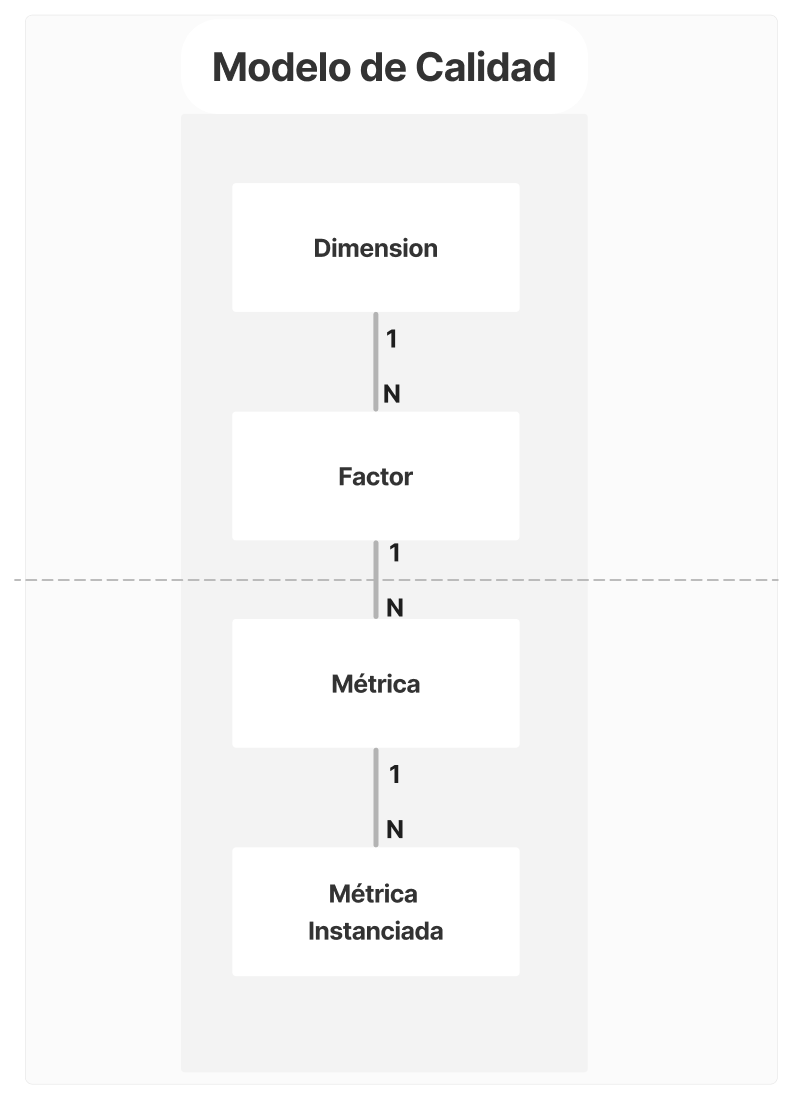
\includegraphics[width=\linewidth]{modelo.png}
  \caption{Modelo de Calidad} 
  \Description{Modelo de Calidad.}
\end{figure}



\begin{itemize}
    \item \textbf{Dimensiones de calidad:} se caracteriza mediante múltiples dimensiones, que ayudan a clasificar los datos. Una dimensión captura un aspecto de alto nivel de la calidad.
    \item \textbf{Factores de calidad}: un factor representa un aspecto particular de una dimensión de calidad, por ejemplo, la precisión de los datos implica corrección semántica, corrección sintáctica y precisión de los datos. Pueden haber varios factores para la misma dimensión; cada factor se adapta mejor a un problema o tipo de sistema en particular.
    \item \textbf{Métricas de calidad: }una métrica es un instrumento utilizado para medir un factor de calidad específico, por ejemplo, el porcentaje de datos del sistema que coinciden con los datos del mundo real es una métrica para la corrección semántica. Pueden haber varias métricas para el mismo factor de calidad.
    \item \textbf{Métodos de calidad:} un método es un proceso que implementa una métrica de calidad. Se definen dos tipos de métodos: (i) métodos de medición, que calculan la calidad de un objeto midiéndolo directamente (por ejemplo, contando el número de valores nulos en una tupla), y (ii) métodos de agregación, que calculan la calidad de un objeto compuesto mediante la agregación de valores de calidad de las partes del objeto (por ejemplo, calcular la precisión de una tabla promediando la precisión de sus tuplas). Pueden haber varios métodos para implementar la misma métrica.
\end{itemize} 

\footnote{Definiciones disponibles en https://eva.fing.edu.uy/}
\subsubsection{Especificación del modelo de datos}

La especificación del modelo cubrirá los datos de \textbf{Operadores}. 
Se evaluaran la dimensión de \textbf{exactitud}  y \textbf{ unicidad}.  Las preguntas a formular en general son relacionadas con 
\begin{itemize}
    \item ¿Estos datos son lo suficientemente precisos para nuestras necesidades?
    \item ¿El nivel de detalle de los datos es adecuado?
    \item ¿Estos datos se corresponden con el mundo real?
    \item ¿Estos datos tienen errores?
    \item ¿El formato de presentación de los datos es correcto? ¿Es estándar?
    
\end{itemize}

\subsubsection{Factores a Evaluar}
Los tres factores a evaluar en este trabajo son los siguientes: 


    \textbf{\textit{Factor 1:}} \textbf{Exactitud semántica (Semantic accuracy)}, respondiendo a ¿Los datos se corresponden con la realidad?
Eventualmente los datos pueden  no corresponden a ningún estado del mundo real y/o a estado equivocado del mundo real y/o  con errores en algunos atributos.
    
    \textit{\textbf{Factor 2: }}\textbf{Exactitud sintáctica} \textbf{(Syntactic accuracy)}: respondiendo a ¿Los datos tienen errores sintácticos o de formato?
    
Eventualmente los datos podrían presentar: 
\begin{itemize}
    \item Errores de valores: Valores fuera de rango, errores ortográficos y de tipeo. 
    \item Errores de estandarización: Valores que no tienen el formato esperado.
    |\item Valores embebidos: Valores que corresponden a múltiples atributos.
\end{itemize}
\vfill

\begin{figure*}[h]
  \label{fig:especificaciondisenioBD}
  \centering
  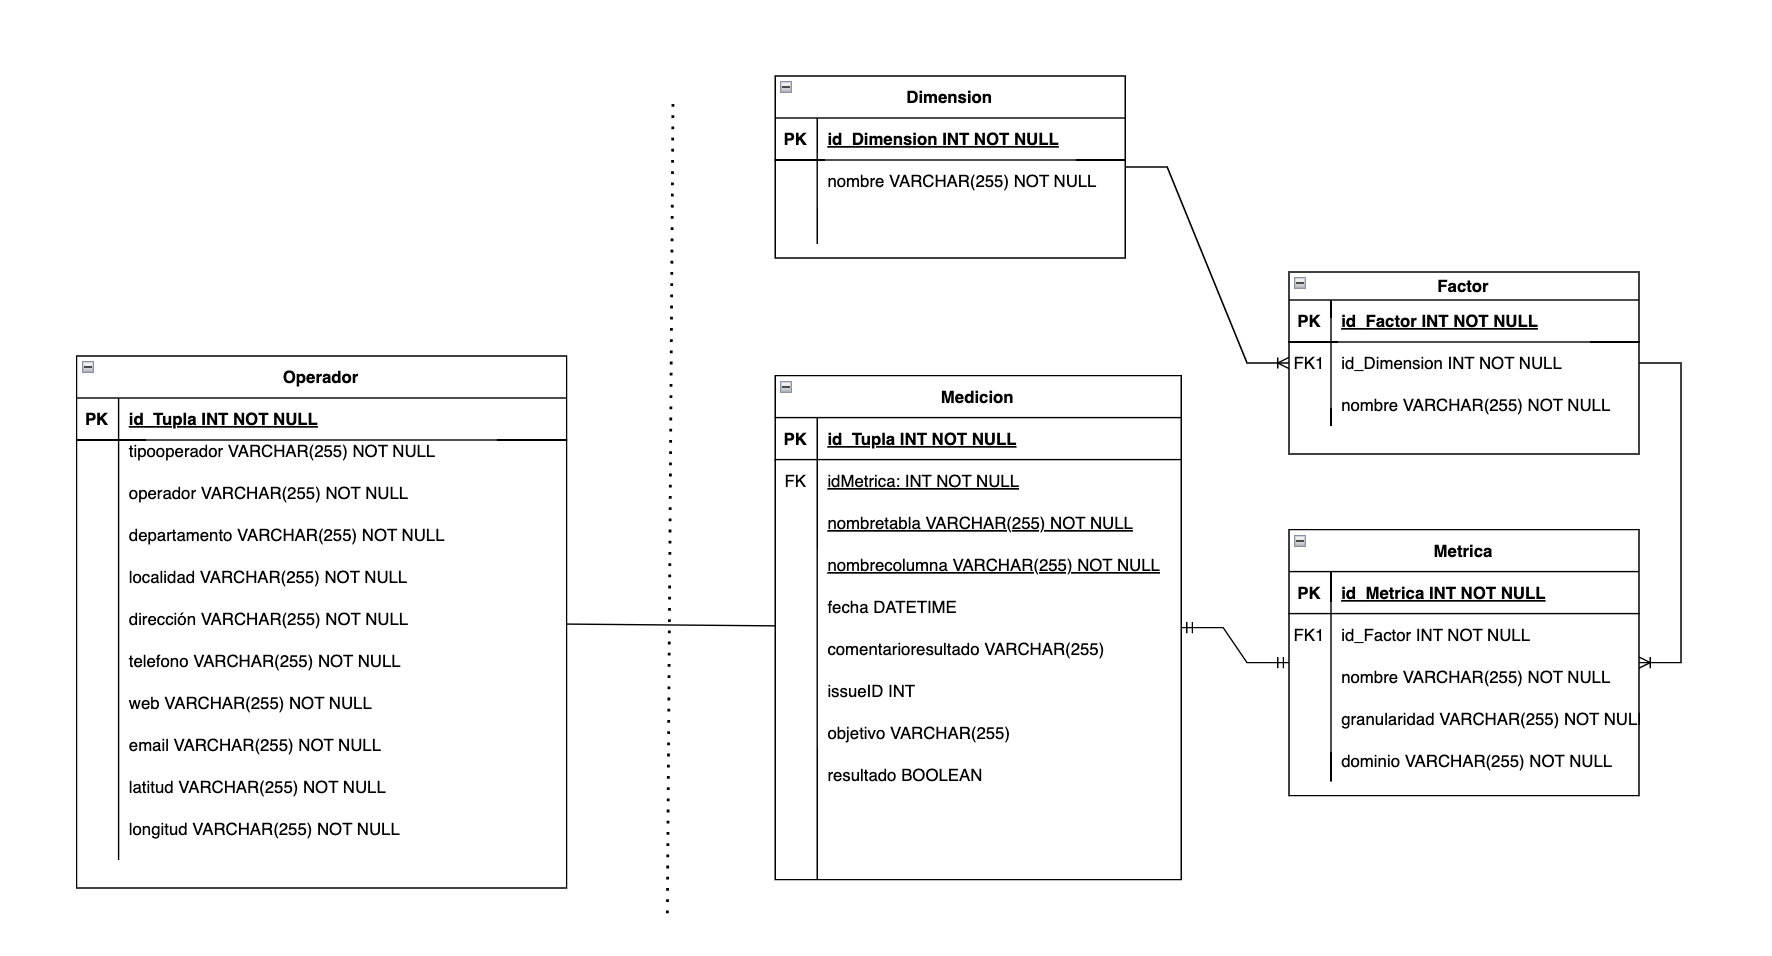
\includegraphics[width=\linewidth]{BD.png}
  \caption{Especificación de diseño de BD de almacenamiento de medidas de calidad obtenidas en la medición} 
  \Description{BD de almacenamiento de medidas de calidad obtenidas en la medición.}
\end{figure*}



\textit{Preguntas 
asociadas a los factores de calidad}

\begin{enumerate}
    \item ¿Las categorías de los operadores se corresponden con los que estan regulados por el Ministerio? (Exactitud semántica).
    \item ¿Las direcciones de mail son correctas? (Exactitud sintáctica).
    \item ¿Los telefonos de contacto de los operadores son números válidos? (Exactitud sintáctica).
    \item ¿La geolocalización es precisa ? (Precisión)
    \item ¿Los operadores estan duplicados?
\end{enumerate}

\subsubsection{Aspectos a evaluar y métricas instanciadas}
En la Tabla~\ref{tab:modelometrica} se presentan los aspectos a evaluar. En particular se seleccionaron las métricas M1,M2,M3 de exactitud sintáctica, semántica y precisión correspondientemente y M4 respecto de unicidad (no duplicación). 
Las métricas variaron desde la verificación de formato, diccionario de datos, cantidades decimales hasta el ratio de no duplicados. 
Los niveles de granularidad fueron a nivel de celda y tabla.

En la Tabla~\ref{tab:modelometricainstanciada} se presentan las métricas instanciadas. Las métricas M1, M2, M3 y M4 fueron instanciadas sobre el dataset de Operadores. La métrica M1, refería a el mail, url y télefono de los cuales se verifico la correctitud del formato de mail estandar. Las otras métricas instanciadas referían a tipo de operador, departamento, longigud y latitud. 
\begin{table*}
  \caption{Modelo de Metricas}
  \label{tab:modelometrica}
  \begin{tabular}{llp{3cm}p{4cm}p{3cm}p{1cm}}
    \toprule
     MetricaID &Dimensión & Factor & Métrica General & Métrica Definición & \\
    \midrule
    M1 & Exactitud & Exactitud sintáctica  & Verificación de Formato  &  granularidad: celda, dominio:{0,1}\\
    M2 & Exactitud& Exactitud semántica  & Diccionario de Datos  &  granularidad: celda, dominio:{0,1}\\
    M3 & Exactitud& Precisión & Cantidad Decimales  &  granularidad: columna, dominio:{0,1}\\
    M4 & Unicidad & No-duplicación &  Ratio no-duplicados &  granularidad: tabla, dominio{\%}\\

  \bottomrule
\end{tabular}
\end{table*}

\begin{table*}
  \caption{Metricas Instanciadas }
  \label{tab:modelometricainstanciada}
  \begin{tabular}{lp{4cm}p{5cm}p{7cm}p{1cm}}
    \toprule
         MetricaID &   Metrica Instanciada &  Objetivo\\
    \midrule
       M1 &   Operadores.mail & Verificar que es el formato correcto de email \\
         &   Operadores.web & Verificar que es el formato correcto de url \\
         &   Operadores.telefono & Verificar si la caracteristica corresponde con el Departamento\\
     \midrule
        M2 &   Operadores.tipooperador & Verificar si el operador esta en la lista de operadores clasificadas por el Ministerio de Turismo\\
         &   Operadores.departamento & Verificar si el departamento esta en la lista de departamentos de Uruguay\\ 
      \midrule
        M3 &   Operadores.longitud & Verificar 4 dígitos decimales  y > 0 \\
         &   Operadores.latitud & Verificar 4 dígitos decimales  y > 0 \\ 
       \midrule
        M4 &   Operadores & Verificar no duplicados.\\
  \bottomrule
\end{tabular}
\end{table*}

\subsection{Especificación de BD de almacenamiento de medidas de Calidad}



En la Figura 1 se presenta el diseño de especificación de la base de datos donde se almacenarían las medidas de calidad obtenidas en la medición estableciendo la medición, factor y métrica asociada a la estructura de Operador. 



Las medidas de calidad se almacenarán en  archivos planos Google Drive y las distintas versiones de cambios se reportarán en el repositorio de GIT \footnote{\url{https://github.com/aadorian/cibse_taller}} y
URL de Google Drive \footnote{\url{https://docs.google.com/spreadsheets/d/1lcC7mO1O9nn1oqlAxfEHz2H4fmPsvC66tqk4KZLnMg8/edit?usp=sharing}}


Los archivos fuentes de datos se trabajarán con los CSV que fueron provistos en formato original. Los archivos de trabajos de ejecución de la ejecución se realizarán en DataCleaner versión  5.8.1 (si bien no se realizará la etapa de limpieza, transformación y análisis posterior).  La ejecución de los mismos será exploratoria. 


Evaluamos los datos de Operadores  turísticos \footnote{https://www.gub.uy/tramites/inscripcion-operador-turistico} por el hecho de su relevancia en el vínculo entre el turismo receptivo y emisivo .
La actividad de operadores turísticos esta a su vez regulada  por el registro de operadores en \url{https://www.gub.uy/tramites/inscripcion-operador-turistico}. 



\section{Tablas resultados de emisivos, receptivos y operadores}



En la Tabla~\ref{tab:emisivos} se presenta el resumen correspondiente al data profiling de  ``\verb|emisivos|''

\begin{table}
  \caption{Resumen del data profiling de emisivos}
  \label{tab:emisivos}
  \begin{tabular}{lcl}
    \toprule
    Estadística del dataset&Frecuencia&\\
    \midrule
    Número de variables & 43  \\
    Número de observaciones & 20602  \\
    Celdas faltantes &  7241 \\
    Celdas faltantes (\%)& 0.8\%  \\
    \midrule
    Variables numéricas & 29  \\
    Variables categóricas & 14   \\
    \midrule
    Alertas & 21   \\ 
  \bottomrule
\end{tabular}
\end{table}


En la Tabla~\ref{tab:receptivos} se presenta el resumen correspondiente al data profiling de ``\verb|receptivos|''.

\begin{table}
  \caption{Resumen del data profiling de receptivos}
  \label{tab:receptivos}
  \begin{tabular}{lcl}
    \toprule
    Estadística del dataset&Frecuencia&\\
    \midrule
    Número de variables & 48  \\
    Número de observaciones &  48388 \\
    Celdas faltantes &  	25596 \\
    Celdas faltantes (\%)& \%  	1.1\%\\
    \midrule
    Variables numéricas &  	29 \\
    Variables categóricas &  19  \\
    \midrule
    Alertas &  27  \\ 
  \bottomrule
\end{tabular}
\end{table}

\textit{Nota:} Las alertas de la Tabla~\ref{tab:receptivos} corresponden a alta cardinalidad, desvalance, valores faltantes, ceros y alta varianza.


En la Tabla~\ref{tab:operadores} se presenta el resumen correspondiente al data profiling de ``\verb|operadopres|'' Turísticos.

\begin{table}
  \caption{Resumen del data profiling de Operadores}
  \label{tab:operadores}
  \begin{tabular}{lcl}
    \toprule
    Estadística del dataset&Frecuencia&\\
    \midrule
    Número de variables &  10 \\
    Número de observaciones & 	3288  \\
    Celdas faltantes &  	1	 \\
    Celdas faltantes (\%)& < 0.1\%\\
    Datos duplicados & 98 \\
    Datos duplicados(\%)& 3.0\% \\
    \midrule
    Variables numéricas &  0	 \\
    Variables categóricas & 10   \\
    \midrule
    Alertas &  11  \\ 
  \bottomrule
\end{tabular}
\end{table}




\textit{Nota:} Las alertas de la Tabla~\ref{tab:emisivos} corresponden a alta cardinalidad, valores faltantes, ceros y alta varianza.

\textit{Nota:} Las alertas de la Tabla~\ref{tab:operadores} corresponden a alta cardinalidad, duplicados y desvalance.

\begin{table}
  \caption{Tipos }
  \label{tab:tipos}
  \begin{tabular}{lcl}
    \toprule
    Estadística del dataset&Frecuencia&\\
    \midrule
    Número de variables &  10 \\
    Número de observaciones & 	3288  \\
    Celdas faltantes &  	1	 \\
    Celdas faltantes (\%)& < 0.1\%\\
    Datos duplicados & 98 \\
    Datos duplicados(\%)& 3.0\% \\
    \midrule
    Variables numéricas &  0	 \\
    Variables categóricas & 10   \\
    \midrule
    Alertas &  11  \\ 
  \bottomrule
\end{tabular}
\end{table}


\vfill



La creación de un diccionario de datos de categorías correspondientes a las publicadas en el ministerio permitió cotejar con los registros ingresados.

\begin{table}[!h]
   \caption{Nivel de riesgo calidad, umbral establecido en categorías: alto, medio y bajo }
  \label{tab:nivelcalidad}
  \begin{tabular}{lcl}
    \toprule
    Nivel &Rango&\\
    \midrule
    alto & >90\% de los datos contienen errores  \\
    medio  &  [60,90]\% de los datos contienen errores\\
    bajo & < 60\% de los datos contienen errores

\end{tabular}
\end{table}

En las Figuras 2 y 3 se presentan los snapshots de ejemplos de ejecución de ydataprofiling y DataCleaner respectivamente. 
En las Figuras 4, 5, 6 y 7 presentadas en el anexo se ilustra los templates utilizados en el diseño de medición de calidad.

\section{Resultados}

 

\subsection{Ejecución de la medición}

La ejecución esta disponible en \footnote{\url{https://docs.google.com/spreadsheets/d/1lcC7mO1O9nn1oqlAxfEHz2H4fmPsvC66tqk4KZLnMg8/edit?usp=sharing}}

En la Tabla \ref{tab:ejecuciontotal} se presenta el resumen de los resultados de medición. 

Nota: las medidas 4.1 y 4.2 correspondientes a latitud, longitud no se realizaron, considerando que el alcance que  problema excede las herramientas de data profiling que tenemos disponibles o que pudimos evaluar, sería interesante utilizar el mapeo de una herramienta de geolocalización que permitiera evaluar de forma automática la misma.

\begin{table}[!h]
  \caption{Resumen de resultados de medición. }
  \label{tab:ejecuciontotal}
  \begin{tabular}{lclll}
    \toprule
    Medida ID & Total &Nivel Riesgo & Sin Datos & Porcentaje \\
    \midrule
    1.1&	1&	bajo&	827 &0.0003\% \\
    1.2	&3285&	alto&	1450	& 99\%	\\
    2.1	& 6	&	bajo&			0.001\% \\
    3.1	&3269&	alto &	0	&99\% \\
    4.1	&	- &-  &-  & -\\
    4.2	&	- &-  &-  & -\\
    5.1	&1283&	bajo & 0 &39\%	\\
    5.2	&2082&	medio & 0 &63\%	\\
    5.1	&2277&	medio & 0 &69\%	\\
  \bottomrule
\end{tabular}
\end{table}

\subsection{Evidencias de ejecución y reporte.}

La ejecución de scripts ``job'' de DataCleaner estan disponibles en \url{https://github.com/aadorian/cibse_taller/tree/main/exec_dataprofiling/jobs}

La visualización de la ejecución en formato HTML esta disponible en \url{https://github.com/aadorian/cibse_taller/tree/main/exec_dataprofiling/results}

La Figura 6 presenta un snapshot de la ejecución de la medición.
\section{Discusión}

\subsection{Evaluación final de la calidad }

La evaluación final de la calidad se presenta en detalle la Tabla \ref{tab:evaluacionfinal1} y \ref{tab:evaluacionfinal2} respectivamente. 
En dichas tablas se presenta un análisis detallado del resultado de cada una de las medidas realizadas y comentarios, así como una posible sugerencia de acciones correctivas. 

\subsection{Análisis de resultados de medición }

Los resultados de medición presentados muestran un grado alto en relación a problemas de calidad. 
Si bien se estableció un umbral arbitrario, si se considerara que los errores de calidad en un rango de aceptación del nivel del 10\% podríamos decir que todas las métricas estarían en frente a la presencia de un alto grado de problemas de calidad de datos. 

El análisis inicial exploratorio de este trabajo dio evidencia del descubrimiento de distintos tipos de errores. Por un lado los correspondiente a datos incompletos, errores de formato y de duplicación entre otros. 

El nivel de confianza en la calidad de datos es de bajo nivel en general. Un análisis mas detallado y ejecución de un diseño mas elaborado permitiría identificar en mejor detalle la calidad de los mismos. 


\subsection{Niveles de Calidad esperados}

Los niveles obtenidos de calidad son bajos a nivel global (se establecieron en la Tabla~\ref{tab:nivelcalidad}). El análisis preliminar de este trabajo permite evidenciar que si los datos básicos de operadores turísticos contienen problemas de calidad, las decisiones basadas en datos que podrían surgir del análisis de los mismos podrían ser incorrectas y eventualmente inexactas. 


\section{Conclusiones}



\begin{table*}
  \caption{Evaluación Final de Calidad}
    \label{tab:evaluacionfinal1}
\begin{tabular}{|c|p{4cm}|p{4cm}|p{4cm}|}
\hline
\textbf{Medida ID}  & \textbf{Nota} & \textbf{Sug. Acción Correctiva} & \textbf{Comentarios} \\ \hline
1.1   & Si bien cumplen en su mayoría con el formato, varios mails están registrados como listas con delimitadores distintos (ejemplo ; o / ). Otros directamente no tienen mail asignado. A su vez, unos con mayúscula. & Unificar a un único formato de minúsculas con una validación de la expresión regular correspondiente al email. En caso de identificar un listado de emails, asignar una estructura adecuada para identificarlos. & Del total de registros 3288, 827 no tienen asignado un valor \\ \hline
1.2   & Varios registros independientemente del formato http:// o https:// no cumplen con el formato estándar de acceso (por ejemplo, hay registros con espacios, caracteres especiales). & Unificar el formato y validar el acceso a la URL mediante un mecanismo semiautomático que permita establecer si la URL está disponible en tiempo real y se corresponde con el sitio web del operador. & Del total de registros 1450 no tienen URL \\ \hline
2.1   & En general los registros están dentro del dominio especificado, si bien no se realizó un análisis exhaustivo del mismo. & Realizar un análisis de que la característica se corresponda con la localidad en la cual se encuentra el operador. &\\ \hline
3.1   & 3269 del total de 3288 de los valores NO coincide con la definición formal del tipo de operador definido por el Ministerio de Turismo. Si bien uno podría mapear, por ejemplo, Inmobiliaria se podría eventualmente ser una Agencia de Viajes, pero podría ser catalogado inicialmente como Prestador servicio Turístico inmobiliario. A su vez, un mismo operador podría prestar varios servicios y esto no está contemplado. & Establecer un identificador que permita sin ambigüedad identificar el tipo de operador y que este corresponda con el asignado como categoría del Ministerio en \url{https://www.gub.uy/tramites/inscripcion-operador-turistico}. Rediseñar el diccionario de categorías. & El total del registro no se corresponden con la descripción exacta del tipo indicado como categoría en el ministerio. A su vez, por ejemplo, la categorización en sí debería ser no ambigua (SALAS DE CONVENCIONES instaladas en Establecimientos Rurales. SALAS DE CONVENCIONES instaladas en Alojamientos Turísticos. SALAS DE CONVENCIONES instaladas en establecimientos que no requieren inscripción en el Registro de Prestadores de Servicios Turísticos). En el registro se reporta SALA DE CONVENCIÓN y no necesariamente está clara a cuál de las tres posibles se refiere. \\ \hline
4.1    & No se realizó una evaluación de latitud / longitud dado el alcance que  problema excede las herramientas de data profing que tenemos disponibles& &\\ \hline
4.2    &  No se realizó una evaluación de latitud / longitud dado el alcance que  problema excede las herramientas de data profing que tenemos disponibles  & &\\ \hline


\end{tabular}
\end{table*}



\begin{table*}[h]
  \caption{Continuación evaluación final de calidad.}
  \label{tab:evaluacionfinal2}
\begin{tabular}{|c|p{4cm}|p{4cm}|p{4cm}|}
\hline
\textbf{Medida ID}  & \textbf{Nota} & \textbf{Sug. Acción Correctiva} & \textbf{Comentarios} \\ \hline
5.1  & 2005 registros son únicos de operadores, y 1283 no son únicos completando asi los 3288 registros existentes & Establecer un criterio de unicidad en el listado.  & Varios registros estan duplicados por tipo de operador teniendo registros como por ejemplo ABITAB  que aparece 182 veces.  \\ \hline
5.2  &  Varios mails estan registrados de forma incorrecta  &  Establecer un criterio de contacto de mail de los operadores & \\ \hline
5.3  & 1011 de los 3288 son registros únicos. Sin embargo hay 2277 no únicos de los cuales 1450 no tienen descripción & Establecer un criterio de unicidad de URL del operador & \\ \hline
\end{tabular}
\end{table*}

En este trabajo se realizó un ejemplo de aplicación de ``data profiling''. 
Se aplicaron técnicas y métodos de análisis de datos para cumplir con los objetivos del trabajo. 
Se especificación de un modelo de calidad de datos para luego ser ejecutado. 
La utilización de dos herramientas como ydata-profiling y Data Cleaner 5.8.1 permitieron realizar la tarea de ejecución del diseño \footnote{https://datacleaner.github.io/downloads}. Se encontraron varios problemas de calidad de datos los cuales no necesariamente son sencillos de identificar a priori. La sistematización de diseño previo y ejecución posterior permitió seguir un proceso interesante. Un análisis mas riguroso y en detalle debería ser necesario para identificar los problemas de calidad de datos existentes. 




%%
%% The acknowledgments section is defined using the "acks" environment
%% (and NOT an unnumbered section). This ensures the proper
%% identification of the section in the article metadata, and the
%% consistent spelling of the heading.
%%
%% The next two lines define the bibliography style to be used, and
%% the bibliography file.


\bibliographystyle{ACM-Reference-Format}
\bibliography{sample-base}

%%
%% If your work has an appendix, this is the place to put it.
\appendix


\section{Snapshot de Herramientas}

\begin{figure*}[h]
  \centering
   \label{fig:ydataprof}
  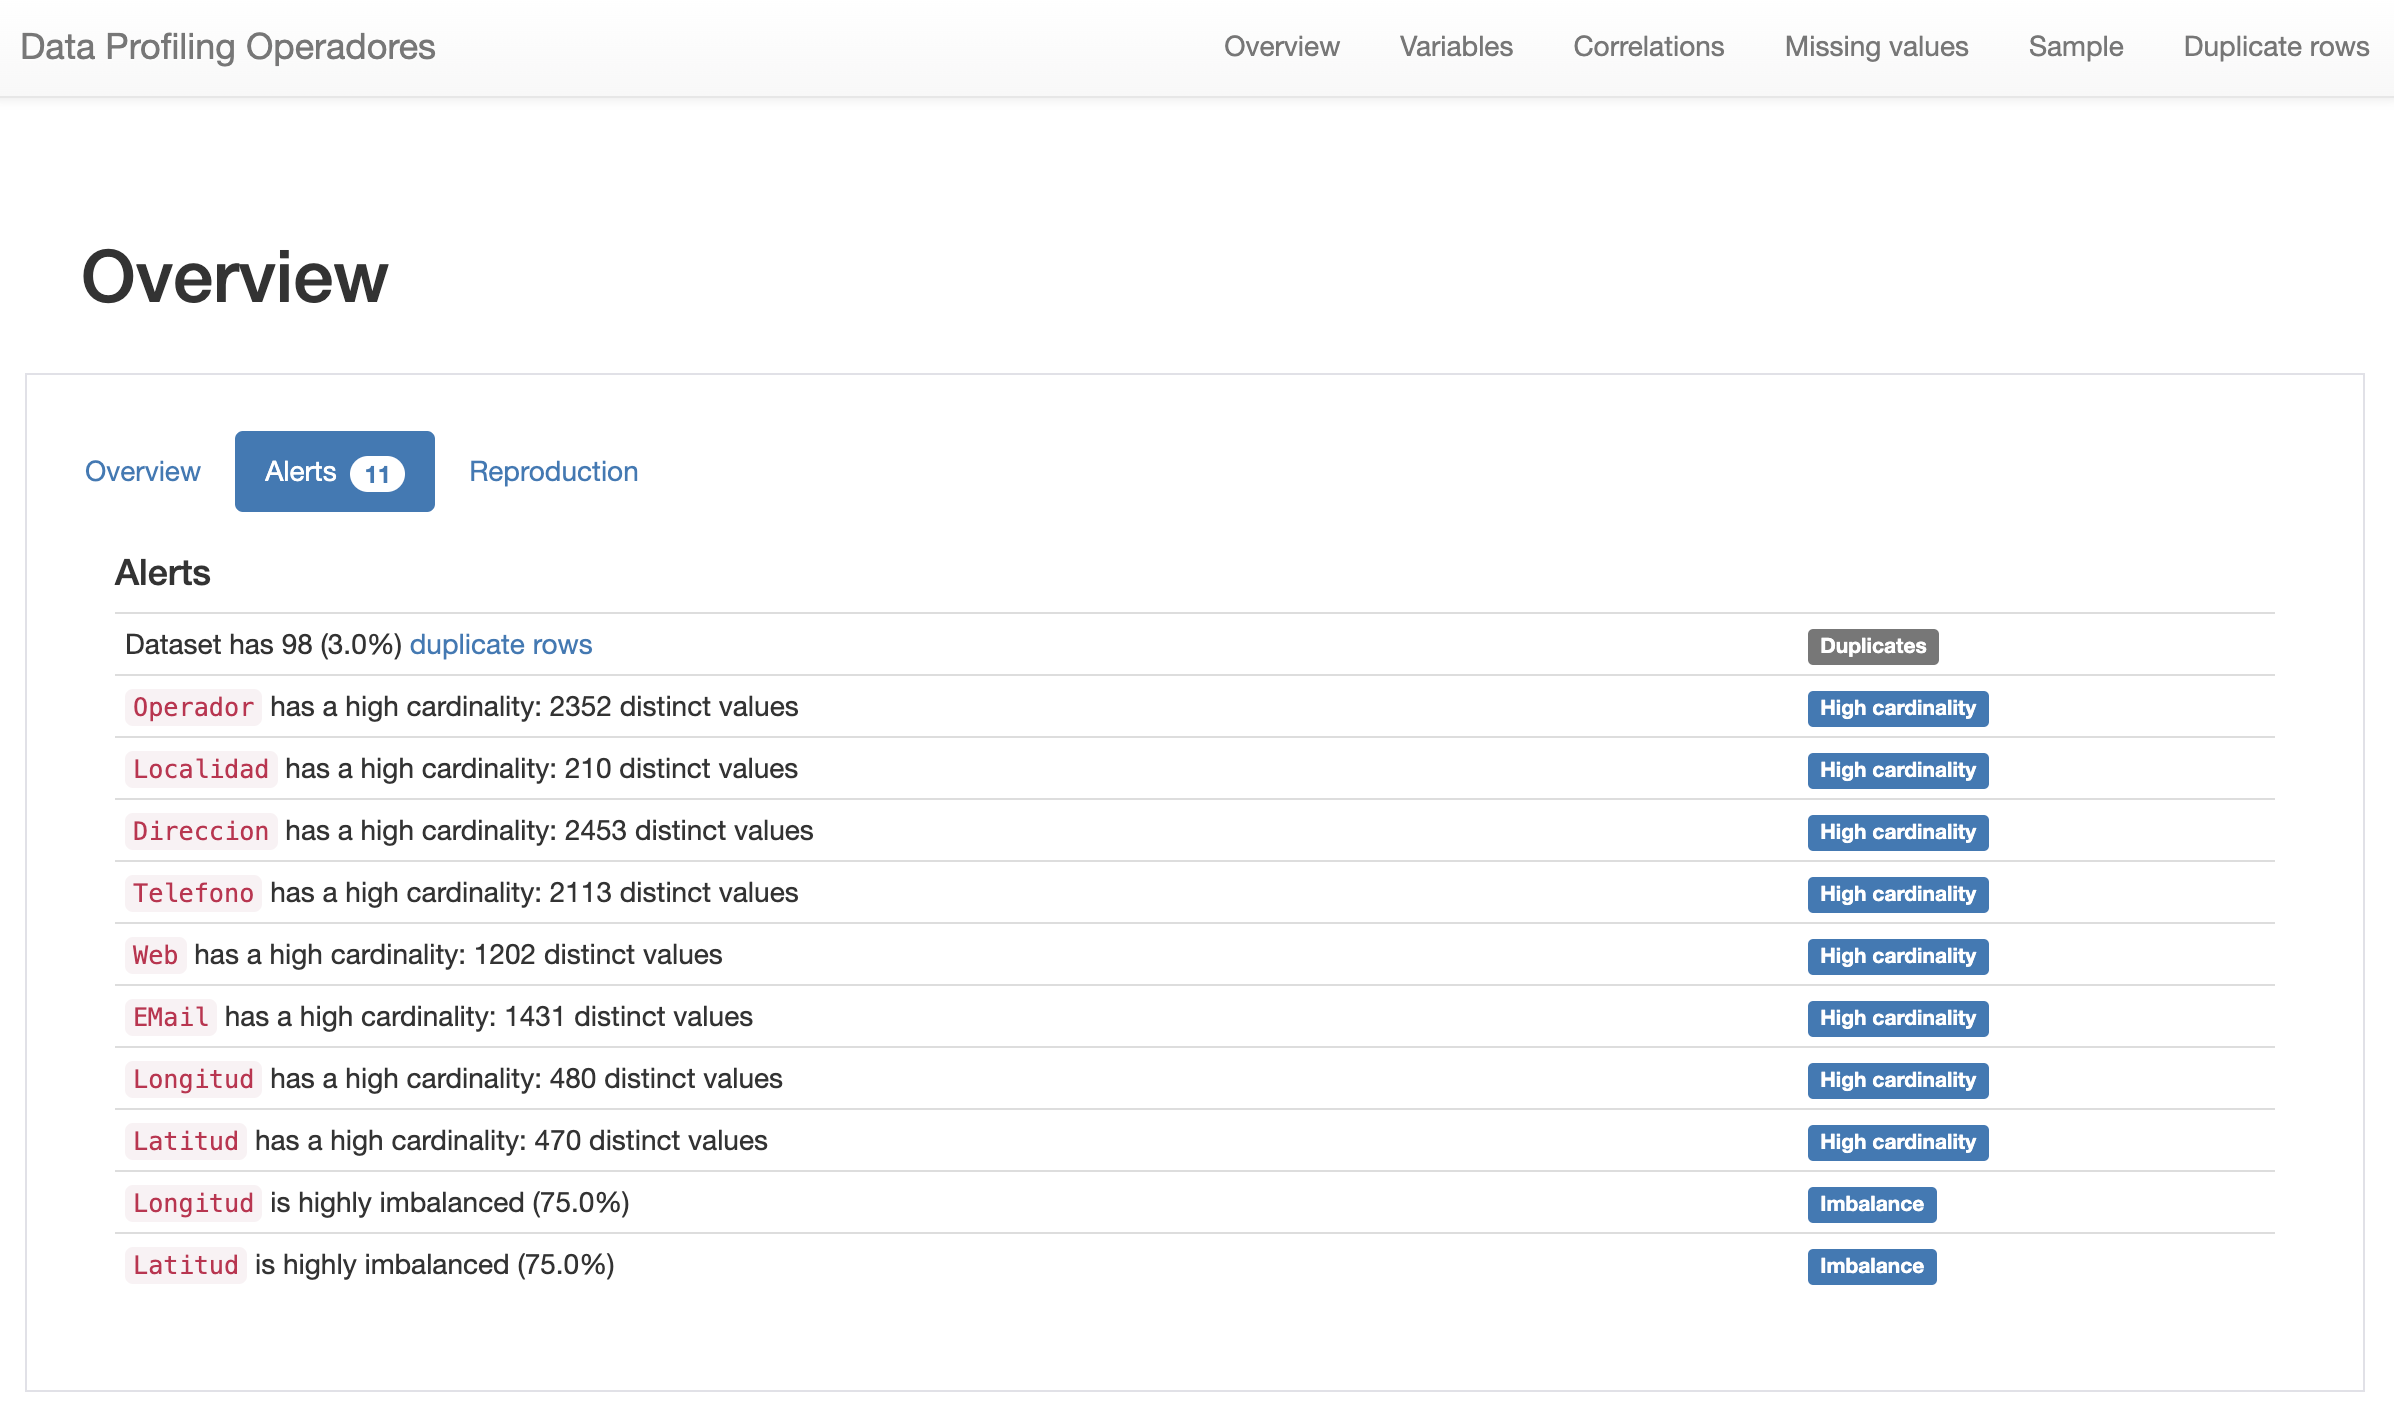
\includegraphics[width=\linewidth]{Overview.png}
  
  \caption{Ejecución exploratoria inicial de Data Profiling Operadores.} 
  \Description{Ejecución exploratoria inicial de Data Profiling Operadores.}
\end{figure*}

\begin{figure*}[h]
  \centering
   \label{fig:datacleanersnapshot}
  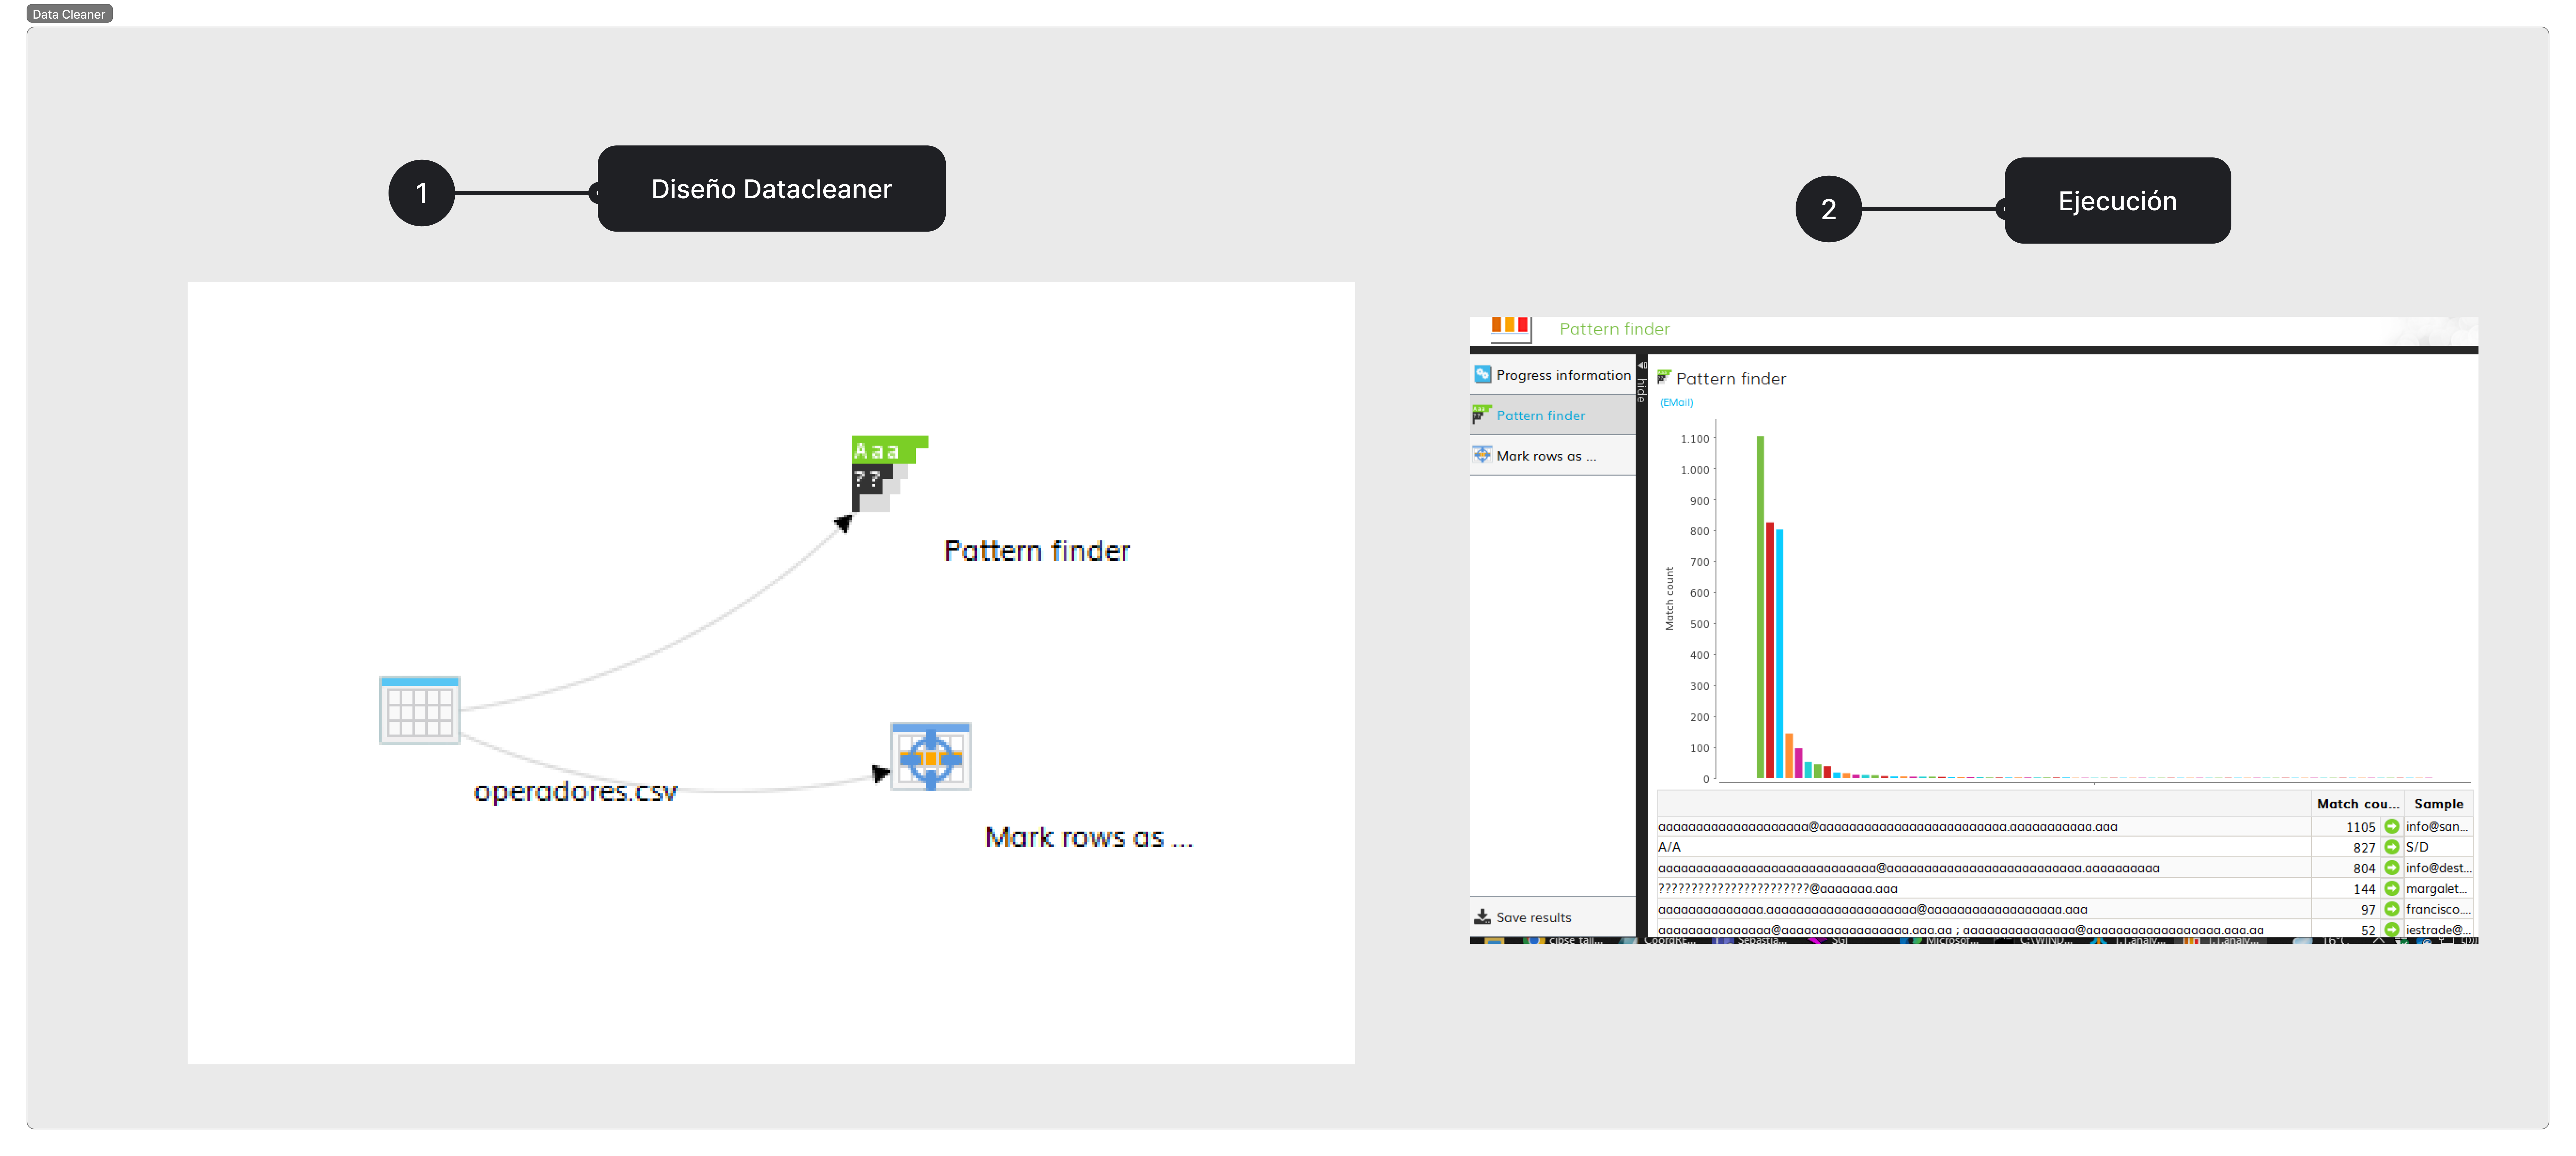
\includegraphics[width=\linewidth]{gui.png}
  \caption{Ejemplo de ejecución de job en DataCleaner} 
  \Description{Ejemplo de ejecución de job en DataCleaner.}
\end{figure*}


\section{Templates de Diseño }
\begin{figure*}[h]
   \label{fig:templateregistro}
  \centering

  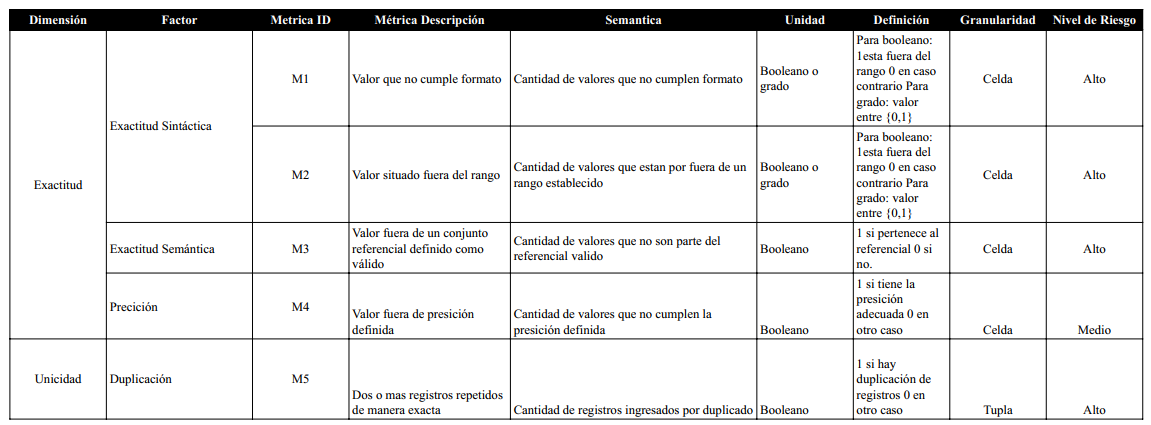
\includegraphics[width=\linewidth]{1.png}
  \caption{Diseño de dimensión, factor y métrica. } 
  \Description{Diseño de dimensión, factor y métrica.}
\end{figure*}

\section{Ejecución de la medición }
\begin{figure*}[h]
   \label{fig:execu}
  \centering

  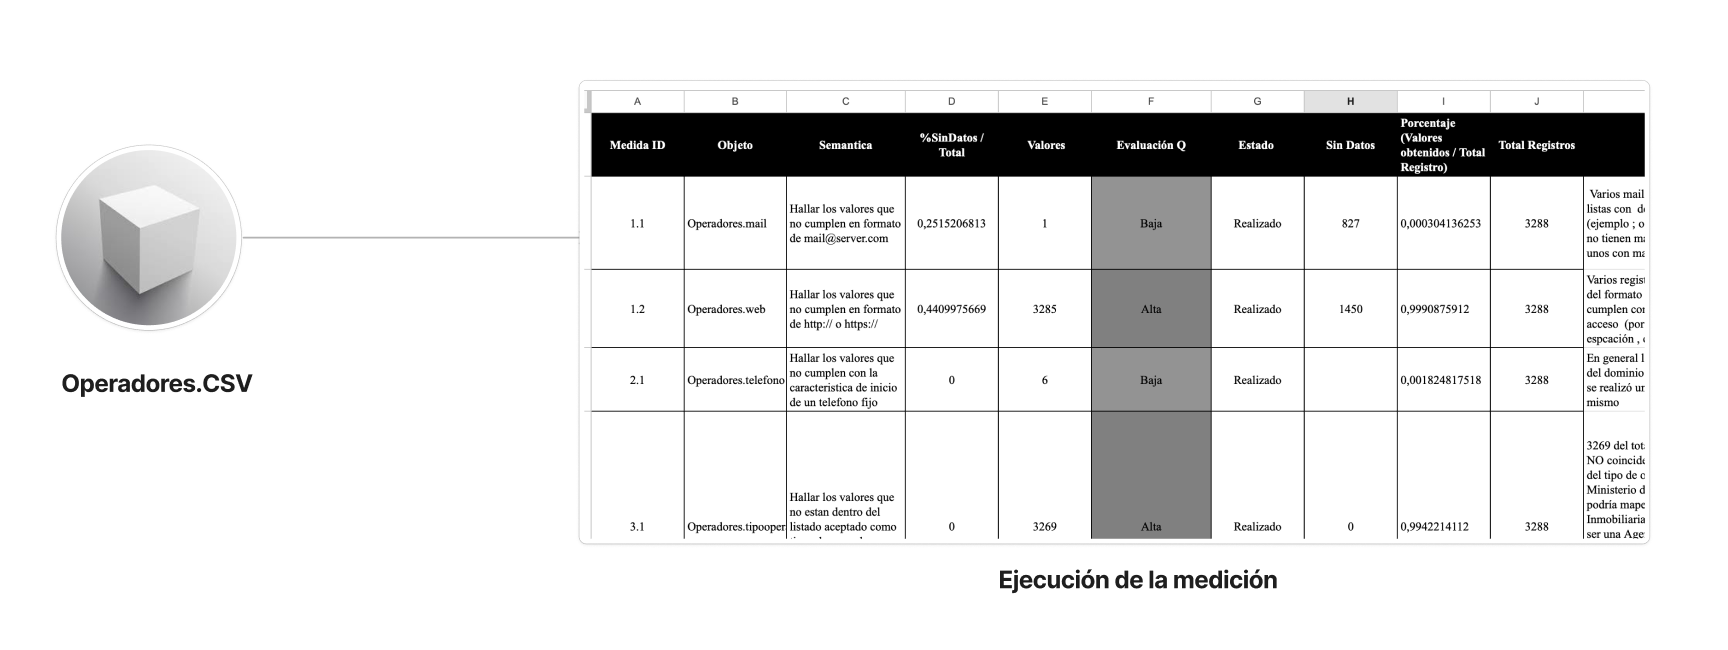
\includegraphics[width=\linewidth]{exe.png}
  \caption{Ejecución de la medición. } 
  \Description{Ejecución de la medición.}
\end{figure*}

\begin{figure*}[h]
   \label{fig:registrometrica}
  \centering

  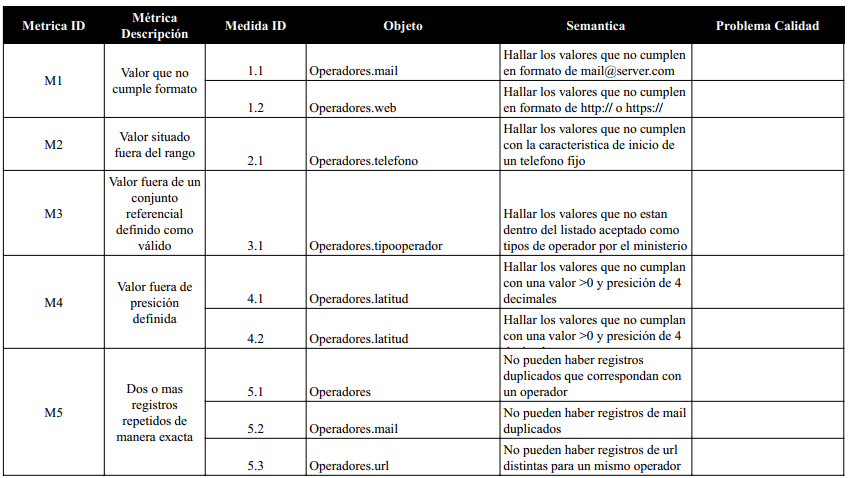
\includegraphics[width=\linewidth]{2.png}
  \caption{Instanciación de Métricas sobre Operadores.} 
  \Description{Instanciación de Métricas sobre Operadores.}
\end{figure*}


\begin{figure*}[!h]
  \centering
   \label{fig:templateresistro}
  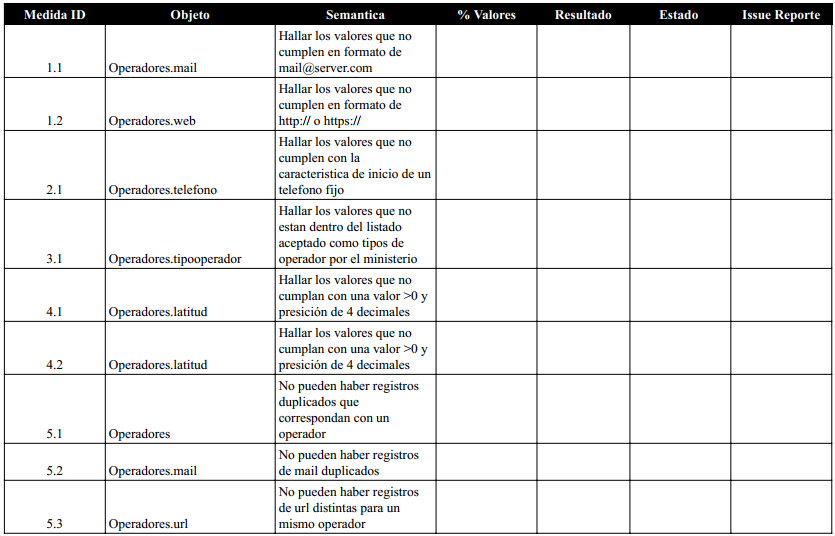
\includegraphics[width=\linewidth]{3.png}
  \caption{Diseño de Template de registro de ejecución } 
  \Description{Diseño de Template de registro de ejecución.}
\end{figure*}

\begin{figure*}[!h]
  \centering
   \label{fig:templateresistro2}
  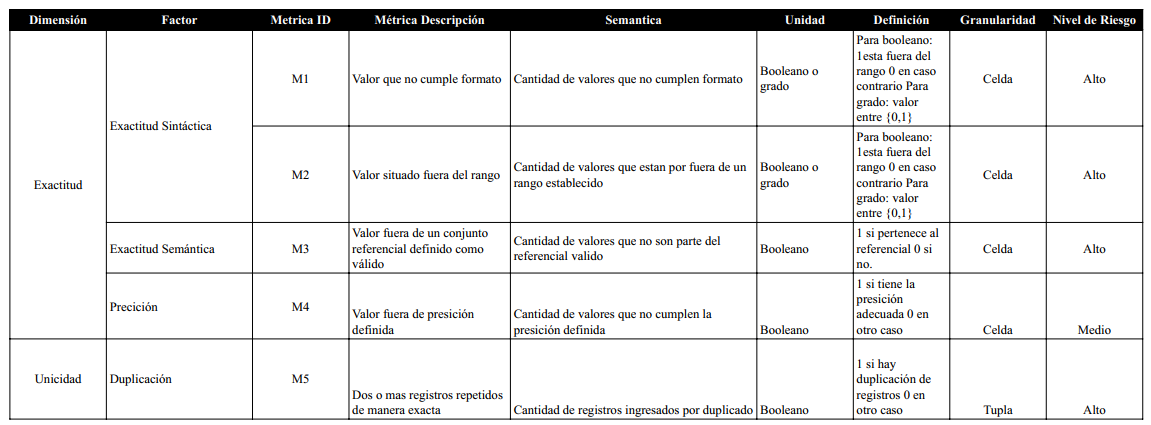
\includegraphics[width=\linewidth]{1.png}
  \caption{Especificación de Registro } 
  \Description{Especificación de Registro.}
\end{figure*}

\subsection{Operadores turísticos categorías }
\begin{enumerate}
 \item AGENCIA DE VIAJES
\item TRANSPORTE TURISTICO
\item ALOJAMIENTO TURÍSTICO
\item PRESTADORES DE SERVICIOS TURISTICOS INMOBILIARIOS
\item TURISMO AVENTURA
\item ESTABLECIMIENTO ENOLÓGICO (Prestan servicios de alojamiento).
\item ESTABLECIMIENTO ENOLÓGICO (NO Prestan servicios de  alojamiento).
SUCURSAL
\item GUIA DE TURISMO
\item ORGANIZADORES PROFESIONALES DE CONGRESOS
\item OBSERVACIÓN DE CETÁCEOS
\item ARRENDADORA DE VEHÍCULOS SIN CONDUCTOR
\item PRESTADORES DE SERVICIOS TURISTICOS RURALES
\item SALAS DE CONVENCIONES instaladas en Establecimientos Rurales.
\item SALAS DE CONVENCIONES instaladas en Alojamientos Turísticos.
\item SALAS DE CONVENCIONES instaladas en establecimientos que no requieren inscripción en el \item Registro de Prestadores de Servicios Turísticos
\end{enumerate}



Fuente: \url{https://www.gub.uy/tramites/inscripcion-operador-turistico}

\footnote{El registro de ejecución y comentarios de evaluación final esta disponible en la siguiente planilla: \url{https://docs.google.com/spreadsheets/d/1lcC7mO1O9nn1oqlAxfEHz2H4fmPsvC66tqk4KZLnMg8/edit?usp=sharing}}



\end{document}
\endinput
%%
%% End of file `sample-sigplan.tex'.
